
\documentclass[12pt]{article}

% Layout.
\usepackage[top=1in, bottom=0.75in, left=1in, right=1in, headheight=1in, headsep=6pt]{geometry}

% Fonts.
\usepackage{mathptmx}
\usepackage[scaled=0.86]{helvet}
\renewcommand{\emph}[1]{\textsf{\textbf{#1}}}

% TiKZ.
\usepackage{tikz, pgfplots}
\usetikzlibrary{calc}
\pgfplotsset{compat = newest}
 
\pgfplotsset{my style/.append style={axis x line=middle, axis y line=
middle, xlabel={$x$}, ylabel={$y$}, axis equal }}

% Misc packages.
\usepackage{amsmath,amssymb,latexsym}
\usepackage{graphicx}
\usepackage{array}
\usepackage{xcolor}
\usepackage{multicol}
\usepackage{enumerate}

% Commands to set various header/footer components.
\makeatletter
\def\doctitle#1{\gdef\@doctitle{#1}}
\doctitle{Use {\tt\textbackslash doctitle\{MY LABEL\}}.}
\def\docdate#1{\gdef\@docdate{#1}}
\docdate{Use {\tt\textbackslash docdate\{MY DATE\}}.}
\def\doccourse#1{\gdef\@doccourse{#1}}
\let\@doccourse\@empty
\def\docscoring#1{\gdef\@docscoring{#1}}
\let\@docscoring\@empty
\def\docversion#1{\gdef\@docversion{#1}}
\let\@docversion\@empty
\makeatother

% Headers and footers layout.
\makeatletter
\usepackage{fancyhdr}
\pagestyle{fancy}
\fancyhf{} % Clears all headers/footers.
\lhead{\baselineskip 30pt
%\emph{\@doctitle\hfill\@docdate}
\emph{\@docdate\hfill\@doctitle}
\ifnum \value{page} > 1\relax\else\\
\emph{Name: \rule{3.5in}{1pt}\hfill \@docscoring}\fi}
\rfoot{\emph{\@docversion}}
\lfoot{\emph{\@doccourse}}
\cfoot{\emph{\thepage}}
\renewcommand{\headrulewidth}{0pt}%
\makeatother

% Paragraph spacing
\parindent 0pt
\parskip 6pt plus 1pt

% A problem is a section-like command. Use \problem{5} to
% start a problem worth 5 points.
\newcounter{probcount}
\newcounter{subprobcount}
\setcounter{probcount}{0}
\newcommand{\problem}[1]{%
\par
\addvspace{4pt}%
\setcounter{subprobcount}{0}%
\stepcounter{probcount}%
\makebox[0pt][r]{\emph{\arabic{probcount}.}\hskip1ex}\emph{[#1 points]}\hskip1ex}
\newcommand{\thesubproblem}{\emph{\alph{subprobcount}.}}

% Subproblems are an enumerate-like environment with a consistent
% numbering scheme. 
% Use \begin{subproblems}\item...\item...\end{subproblems}
\newenvironment{subproblems}{%
\begin{enumerate}%
\setcounter{enumi}{\value{subprobcount}}%
\renewcommand{\theenumi}{\emph{\alph{enumi}}}}%
{\setcounter{subprobcount}{\value{enumi}}\end{enumerate}}

% Blanks for answers in normal and math mode.
\newcommand{\blank}[1]{\rule{#1}{0.5pt}}
\newcommand{\mblank}[1]{\underline{\hspace{#1}}}
\def\emptybox(#1,#2){\framebox{\parbox[c][#2]{#1}{\rule{0pt}{0pt}}}}

% Misc.
\renewcommand{\d}{\displaystyle}
\newcommand{\ds}{\displaystyle}
\def\bc{\begin{center}}
\def\ec{\end{center}}
\def\be{\begin{enumerate}}
\def\ee{\end{enumerate}}


\doctitle{Math F251X: Quiz 3}
\docdate{September 12, 2024}
\doccourse{UAF Calculus I}
\docversion{v-1 async}
\docscoring{\blank{0.8in} / 25}
\begin{document}
\emph{Please circle your instructor's name:} \hfill Leah Berman  \hfill   Jill Faudree \hfill James Gossell \\

There are 25 points possible on this quiz. Any outside materials (textbook, course notes, calculator) are not allowed.  \emph{For full credit, show all work in a way someone else can follow it.} 
\begin{enumerate}
\item (13 points) The graph of a function $H(x)$ is shown below. %has domain $(-\infty,2)\cup(2,\infty)$ and has a vertical asymptote at $x=2.$ 
Use the graph of $H(x)$ to answer each question below. If the limit is infinite, indicate that with $\infty$ or $-\infty.$ If the value does not exist or is undefined, write {\sf DNE}.\\

\begin{center}
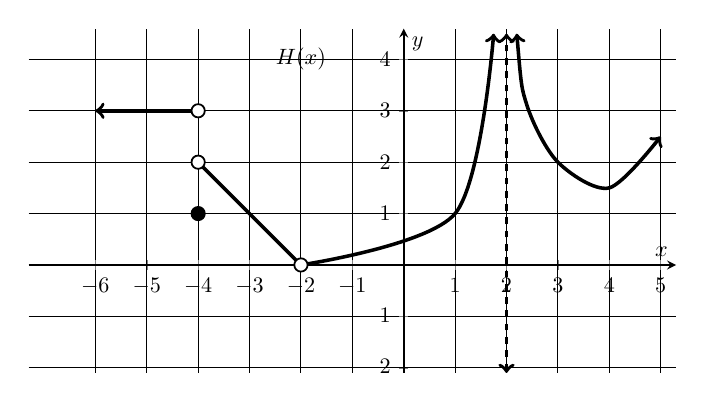
\begin{tikzpicture}[scale = .8]
\begin{axis}[scale=1.5, thick, my style, xtick={-6,-5,-4,...,5}, ytick={-2,-1,1,2,...,4},
xmin=-7.3, xmax=5.3, ymin=-2.1, ymax=4.6, minor y tick num=0,
        minor x tick num=0, mark size=3.0pt, grid=both, grid style={ thin, black, %dashed
        }, axis equal image]
% %%asymptote
%\addplot[dashed,<->, ultra thick] coordinates {(-2,-1) (-2,6.2)}; 
\addplot[dashed,<->, ultra thick] coordinates {(2,-2.1) (2,4.5)};       
%%points solid
\addplot[mark=*,only marks] coordinates {(-4,1)};
%%points open
\addplot[mark=*,fill=white,only marks] coordinates {(-4,2)(-4,3)(-2,0)};
%%Curves
%\addplot[<-,ultra thick, smooth, variable=\x, samples=100, domain=-3:-2.9] plot(\x,{1/(\x+2)^2 - 0.333});
\addplot[ultra thick, smooth, <-] coordinates {(-6,3)(-4,3)};
\addplot[ultra thick, smooth, -] coordinates {(-4,2)(-2,0)};

\addplot[ultra thick, smooth, ->] coordinates {(-2,0)(1,1)(1.75,4.5)};
%\addplot[ultra thick, smooth] coordinates {(-2,2) (1,5)};
% \addplot[->,ultra thick, smooth, variable=\x, samples=100, domain=1:6] plot(\x,{(-0.15)*(\x -1)*(\x -1)+5});   

\addplot[ultra thick, smooth, <->] coordinates {(2.2, 4.5)(2.4, 3.1)
(3, 2)(4,1.5)(5,2.5)} ;

%\addplot[ultra thick, smooth, ] coordinates {(-2,2)(1,5)}; 
%\addplot[ultra thick, smooth, ->] (1,5) parabola bend (4,1) (6,6);

\node at (-2,4)  {$H(x)$};
\end{axis}

\end{tikzpicture}
\end{center}

\begin{enumerate}
\begin{multicols}{3}
\item $\d{\lim_{x \to\ -2^{-}}H(x)}=\mblank{.5in}$
\item $\d{\lim_{x \to\; -2^+} H(x)=\mblank{.5in}}$
\item $H(-2)=\mblank{.5in}$
%\item $f(5)=\mblank{.5in}$
\end{multicols}
%\vspace{0.1in}
\begin{multicols}{3}
\item $ H(-4)=\mblank{.5in}$
\item $\d{\lim_{x \to\; -4^{+}} H(x)=\mblank{.5in}}$
\item $\d{\lim_{x \to\; -4^{-}} H(x)=\mblank{.5in}}$
\end{multicols}
\begin{multicols}{2}
%\item $\d{\lim_{x \to\; -4} H(x)=\mblank{.5in}}$
\item $\ds{\lim_{x\to 2}H(x)=}$ \blank{.5in}
%\item $\ds{\lim_{x\to 3}H(x)=}$ \blank{.5in}
%\vspace{0.1in}
%\item $H(2) = \mblank{.5in}$%Estimate $H(-1).$ \blank{.5in}
\end{multicols}
\item Based on the information from the graph, write the domain of $H(x)$ using interval notation:

 \hrulefill
\vspace{0.1in}
\item  Observe from the graph that $\d{\lim_{x \to\; 3}H(x)} = 2$. 

Determine $\ds{ \lim_{x \to 3 }\frac{5H(x) -1}{x^{2} H(x)} = }$ \vfill
\vspace{0.1in}
\item List all \emph{$\mathbf{x}$-values} in the set $(-\infty, \infty)$ where the function $H(x)$ is not continuous.%, and classify each value as corresponding to a jump discontinuity, removable discontinuity or an infinite discontinuity.\\
%\vfill

$x = $ \ \hrulefill

\end{enumerate}

%\item (2 points)  If $\d \lim_{x \to -4} f(x) =5$ and $\d \lim_{x \to -4} g(x) =-2$, is it possible to evaluate $\d \lim_{x \to -4} \frac{f(x) + g(x)}{x^{2} f(x)}$? If so evaluate the limit. If not, explain why.
%%\vspace{1in}

\newpage

\item (6 points) Use algebra to evaluate the limits below. You must show your work to earn full credit \emph{and} your work will be graded. (That is, you need to \emph{write your mathematics} clearly and correctly. If you do not write $\ds{\lim_{x \to \ldots} \cdots}$ where it is necessary your answer will not be completely correct.% Use = signs to show things are equal.
)
	\begin{enumerate}
	\item $\d \lim_{x \to 3} \frac{x^2+x-6}{(x+3)^{2}}=$
	\vfill
	\item $\d \lim_{h \to 0} \frac{\frac{4}{h+5} - \frac{4}{5}}{h}=$
	\vfill
%	\item $\d \lim_{x\to -4} \frac{2 x^2+7 x-4}{(x+4)(x+2)}=$
%	\vfill
	\end{enumerate}
	
	
\item (6 points) Let \[f(x)=\begin{cases} \frac{x^2+4 x-5}{(x + 6)(x-1)} & x < 1\\ 3\ln(x)& x \geq 1 \end{cases}.\] Show your work clearly, using limit notation, to answer the following:
\begin{enumerate}
	\item $\d \lim_{x \to 1^-} f(x) = $
	\vspace{1in}
	\item  $\d \lim_{x \to 1^+} f(x) = $
	\vspace{.25in}
	\item  $f(1) = $
	\vspace{.25in}
	\item Based on your answers to parts (a), (b) and (c), {\bf check the true statement(s) below}:
	\begin{multicols}{2}
	\begin{enumerate}[$\Box$]
		\item $f$ is continuous at $x=1$.
		\item $f$ has a removable discontinuity at $x=1$.
		\item $f$ has a jump discontinuity at $x=1$.
		\columnbreak
		\item $f$ has an infinite discontinuity at $x=1$.
		\item None of the above.
	\end{enumerate}
	\end{multicols}
%	\vspace{.5in}
\end{enumerate}
\end{enumerate}
\end{document}